\section{Auswertung}
\label{sec:Auswertung}
Im folgenden wird die Hysteresekurve des verwendeten Magneten bestimmt und die Verschiebung der Wellenlänge berechnet.

\subsection{Hysteresekurve}
In der Abbildung \eqref{fig:Hysterese} ist die Hysteresekurve des verwendeten Magneten zu sehen. Es ist eine Verschiebung der Kurve nach oben zu erkennen, allerdings sind mehrere Bereiche ohne Verschiebung dabei. Das kann durch die Ablesefehler des Feldstroms $I$ erklärt werden.
\begin{align}
  \Delta I = 0.25\, \text{A}
\end{align}
Die Ablesefehler kommen durch die analoge Anzeige zustande.

\begin{figure}
  \centering
  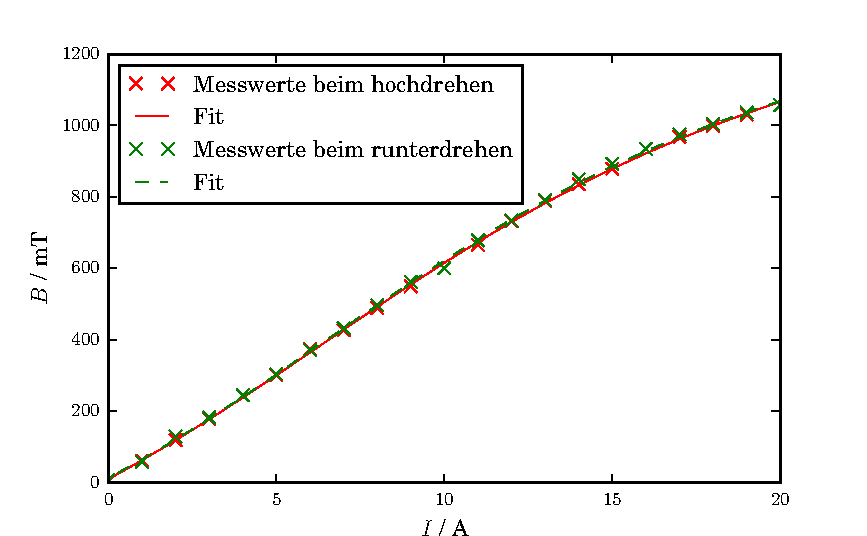
\includegraphics[width=\linewidth]{Bilder/Hysterese.pdf}
  \caption{Die Hysteresekurve des verwendeten Magneten.}
  \label{fig:Hysterese}
\end{figure}


\subsection{Verschiebung der Wellenlänge}
Die Dispersionsgebiete für die blaue und rote Linie lassen sich mit Formel \eqref{eqn:}, zu
\begin{align}
  \Delta\lambda_\text{D,rot} = \frac{(643.8\cdot 10^{-9})^2}{8\cdot 10^{-3}} \cdot \sqrt{\frac{1}{1.4567^2 - 1}} = 0.0489 \cdot 10^{-9}\,\text{m}\ , \\
  \Delta\lambda_\text{D,blau} = \frac{(480.0\cdot 10^{-9})^2}{8\cdot 10^{-3}} \cdot \sqrt{\frac{1}{1.4635^2 - 1}} = 0.0270 \cdot 10^{-9}\,\text{m}\ ,
\end{align}
bestimmen.



\subsubsection{Verschiebung der blauen Linie}

\begin{figure}
  \centering
  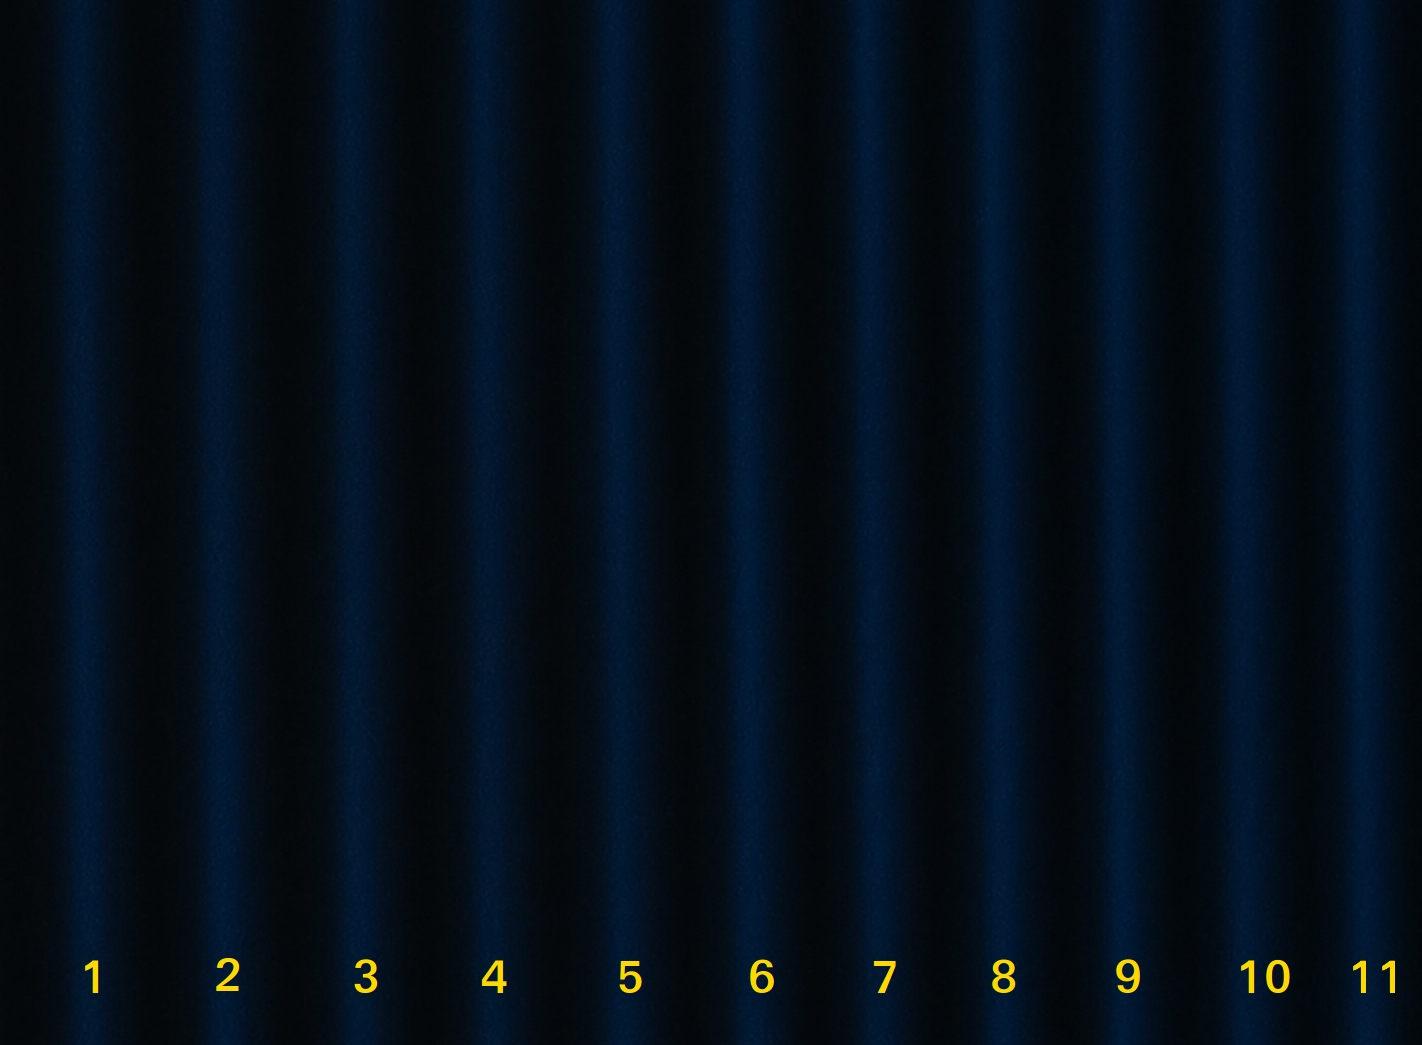
\includegraphics[width=0.8\linewidth]{Bilder/BoB.JPG}
  \caption{Die blaue Linie der Cd-Lampe ohne ein äußeres B-Feld.}
  \label{fig:BoB}
\end{figure}

\begin{figure}
  \centering
  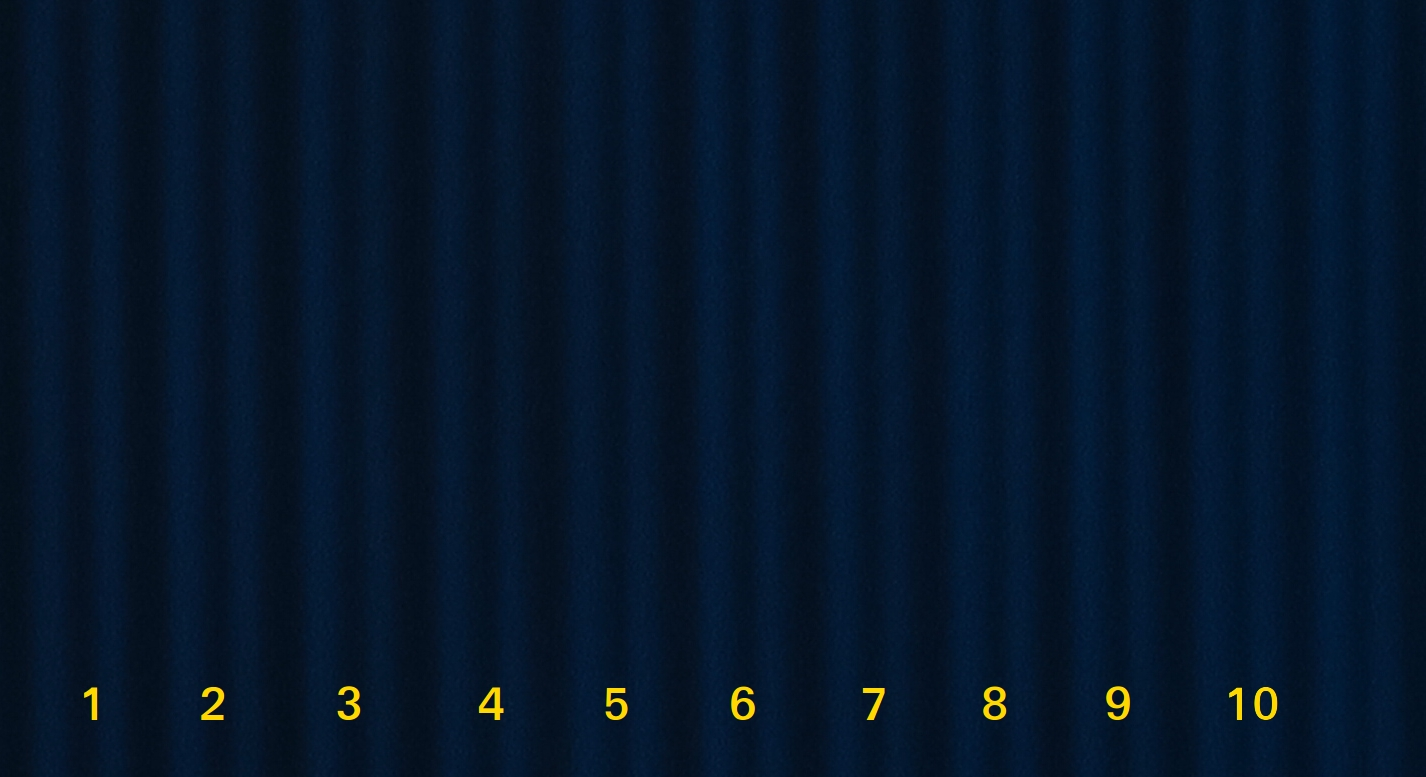
\includegraphics[width=0.8\linewidth]{Bilder/B6ASig.JPG}
  \caption{Die $\sigma$-Komponente der blauen Linie der Cd-Lampe mit einem äußeren B-Feld(6 A).}
  \label{fig:B6ASig}
\end{figure}

\begin{figure}
  \centering
  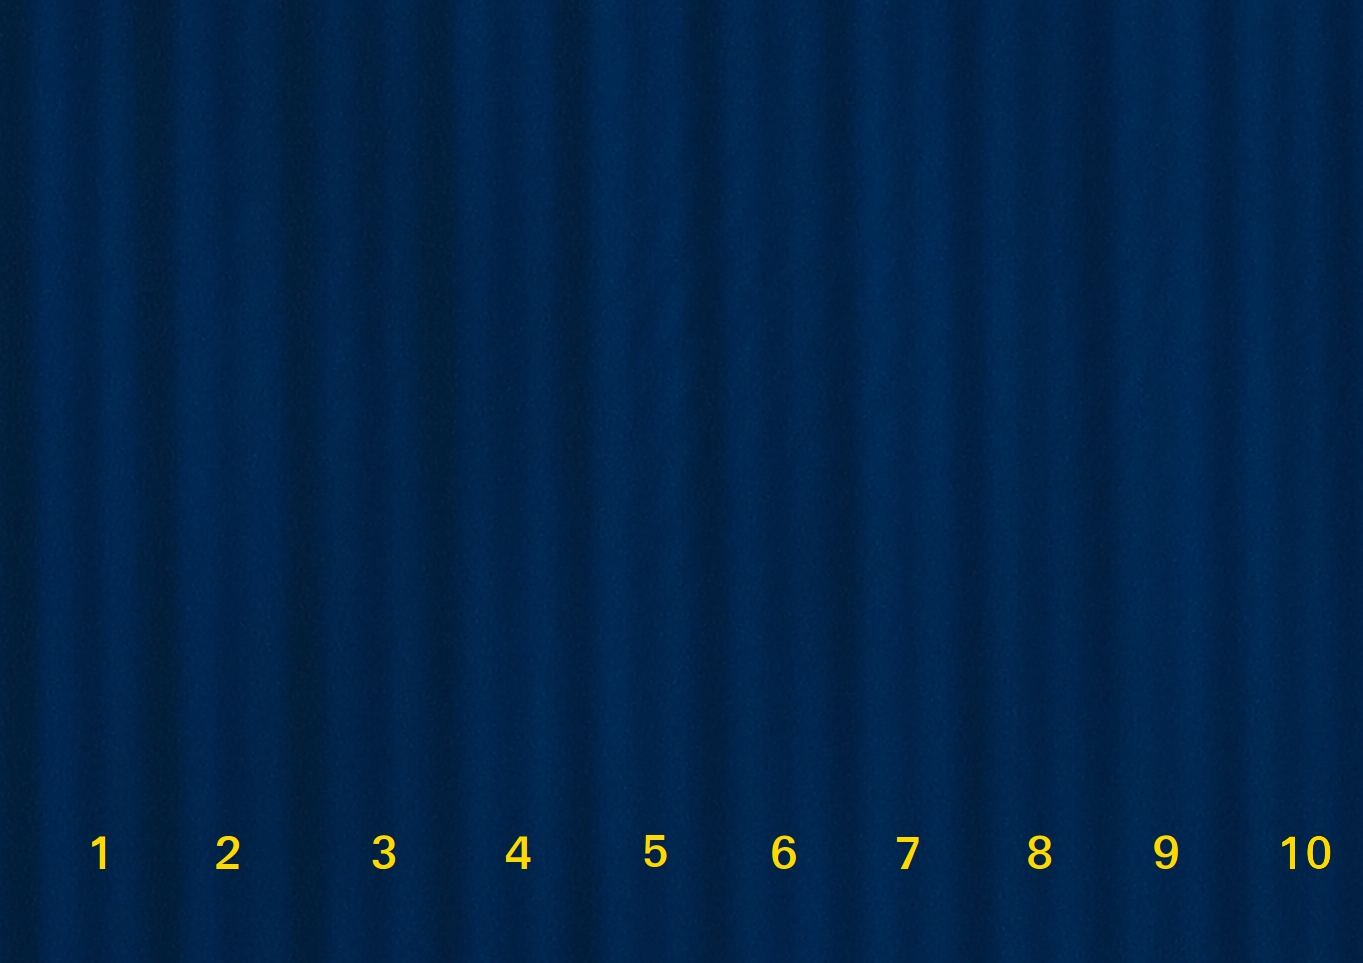
\includegraphics[width=0.8\linewidth]{Bilder/B20APi.JPG}
  \caption{Die $\pi$-Komponente der blauen Linie der Cd-Lampe mit einem äußeren B-Feld(20 A).}
  \label{fig:B20APi}
\end{figure}

Die Werte für die Tabelle \eqref{tab:blau} werden aus den Abbildungen \eqref{fig:BoB} bis \eqref{fig:B20APi} bestimmt.

\begin{table}[H]
  \centering
  \caption{Messwerte für die Berechnung der Verschiebung der blauen Linie.}
  \label{tab:blau}
  \begin{tabular}{c | c c | c c}
    $\Delta$s / Pixel & $\delta$s$_{\sigma}$ / Pixel & $\delta \lambda_{\sigma}$ / $10^{-12}$\,m & $\delta$s$_{\pi}$ / Pixel & $\delta \lambda_{\pi}$ / $10^{-12}$\,m \\
    \hline
    132.7 & 62.7 & 6.37 & 62.0 & 12.33 \\
    135.3 & 56.0 & 5.58 & 65.3 & 10.84 \\
    134.0 & 57.3 & 5.77 & 66.0 & 11.69 \\
    128.7 & 58.7 & 6.14 & 65.3 & 11.86 \\
    130.7 & 55.3 & 5.71 & 61.3 & 11.63 \\
    124.7 & 54.0 & 5.84 & 63.3 & 11.36 \\
    123.3 & 55.3 & 6.05 & 54.0 & 11.88 \\
    122.0 & 52.0 & 5.74 & 57.3 & 11.78 \\
    122.0 & 51.3 & 5.67 & 56.0 & 11.84 \\
    122.0 & 54.7 & 6.04 & 54.0 & 10.84 \\
    \hline
  \end{tabular}
\end{table}


Mit Hilfe der Formel \eqref{eqn:}, der Dispersionsgebiete und der Tabelle \eqref{tab:blau} ergeben sich nach dem mitteln folgende Werte für die Verschiebung $\delta\lambda$:
\begin{align*}
  \delta \lambda_{\sigma,blau} = (\num{5.9 +- 0.2})\cdot 10^{-12}\,\text{m} \\
  \delta \lambda_{\pi,blau} = (\num{6.4 +- 0.3})\cdot 10^{-12}\,\text{m}
\end{align*}



\subsubsection{Verschiebung der roten Linie}



Die Werte für die Tabelle \eqref{tab:blau} werden aus den Abbildungen \eqref{fig:BoB} bis \eqref{fig:B20APi} bestimmt.

\begin{table}[H]
  \centering
  \caption{Messwerte für die Berechnung der Verschiebung der roten Linie.}
  \label{tab:rot}
  \begin{tabular}{c c c}
    $\Delta$s / Pixel & $\delta$s$_{\sigma}$ / Pixel & $\delta \lambda_{\sigma}$ / $10^{-12}$\,m \\
    \hline
    244.0 & 123.0 & 12.33 \\
    240.0 & 106.3 & 10.84 \\
    226.0 & 108.0 & 11.69 \\
    220.0 & 106.7 & 11.86 \\
    213.0 & 101.3 & 11.63 \\
    206.0 & 95.7  & 11.36 \\
    201.0 & 97.7  & 11.88 \\
    193.0 & 93.0  & 11.78 \\
    188.0 & 91.0  & 11.84 \\
    191.0 & 84.7  & 10.84 \\
    \hline
  \end{tabular}
\end{table}


Mit Hilfe der Formel \eqref{eqn:}, der Dispersionsgebiete und der Tabelle \eqref{tab:blau} ergeben sich nach dem mitteln folgende Werte für die Verschiebung $\delta\lambda$:
\begin{align*}
  \delta \lambda_{\sigma,rot} = (\num{11.6 +- 0.4})\cdot 10^{-12}\,\text{m} \\
\end{align*}
